% Options for packages loaded elsewhere
\PassOptionsToPackage{unicode}{hyperref}
\PassOptionsToPackage{hyphens}{url}
\PassOptionsToPackage{dvipsnames,svgnames,x11names}{xcolor}
%
\documentclass[
  letterpaper,
  DIV=11,
  numbers=noendperiod]{scrartcl}

\usepackage{amsmath,amssymb}
\usepackage{lmodern}
\usepackage{iftex}
\ifPDFTeX
  \usepackage[T1]{fontenc}
  \usepackage[utf8]{inputenc}
  \usepackage{textcomp} % provide euro and other symbols
\else % if luatex or xetex
  \usepackage{unicode-math}
  \defaultfontfeatures{Scale=MatchLowercase}
  \defaultfontfeatures[\rmfamily]{Ligatures=TeX,Scale=1}
\fi
% Use upquote if available, for straight quotes in verbatim environments
\IfFileExists{upquote.sty}{\usepackage{upquote}}{}
\IfFileExists{microtype.sty}{% use microtype if available
  \usepackage[]{microtype}
  \UseMicrotypeSet[protrusion]{basicmath} % disable protrusion for tt fonts
}{}
\makeatletter
\@ifundefined{KOMAClassName}{% if non-KOMA class
  \IfFileExists{parskip.sty}{%
    \usepackage{parskip}
  }{% else
    \setlength{\parindent}{0pt}
    \setlength{\parskip}{6pt plus 2pt minus 1pt}}
}{% if KOMA class
  \KOMAoptions{parskip=half}}
\makeatother
\usepackage{xcolor}
\setlength{\emergencystretch}{3em} % prevent overfull lines
\setcounter{secnumdepth}{-\maxdimen} % remove section numbering
% Make \paragraph and \subparagraph free-standing
\ifx\paragraph\undefined\else
  \let\oldparagraph\paragraph
  \renewcommand{\paragraph}[1]{\oldparagraph{#1}\mbox{}}
\fi
\ifx\subparagraph\undefined\else
  \let\oldsubparagraph\subparagraph
  \renewcommand{\subparagraph}[1]{\oldsubparagraph{#1}\mbox{}}
\fi

\usepackage{color}
\usepackage{fancyvrb}
\newcommand{\VerbBar}{|}
\newcommand{\VERB}{\Verb[commandchars=\\\{\}]}
\DefineVerbatimEnvironment{Highlighting}{Verbatim}{commandchars=\\\{\}}
% Add ',fontsize=\small' for more characters per line
\usepackage{framed}
\definecolor{shadecolor}{RGB}{241,243,245}
\newenvironment{Shaded}{\begin{snugshade}}{\end{snugshade}}
\newcommand{\AlertTok}[1]{\textcolor[rgb]{0.68,0.00,0.00}{#1}}
\newcommand{\AnnotationTok}[1]{\textcolor[rgb]{0.37,0.37,0.37}{#1}}
\newcommand{\AttributeTok}[1]{\textcolor[rgb]{0.40,0.45,0.13}{#1}}
\newcommand{\BaseNTok}[1]{\textcolor[rgb]{0.68,0.00,0.00}{#1}}
\newcommand{\BuiltInTok}[1]{\textcolor[rgb]{0.00,0.23,0.31}{#1}}
\newcommand{\CharTok}[1]{\textcolor[rgb]{0.13,0.47,0.30}{#1}}
\newcommand{\CommentTok}[1]{\textcolor[rgb]{0.37,0.37,0.37}{#1}}
\newcommand{\CommentVarTok}[1]{\textcolor[rgb]{0.37,0.37,0.37}{\textit{#1}}}
\newcommand{\ConstantTok}[1]{\textcolor[rgb]{0.56,0.35,0.01}{#1}}
\newcommand{\ControlFlowTok}[1]{\textcolor[rgb]{0.00,0.23,0.31}{#1}}
\newcommand{\DataTypeTok}[1]{\textcolor[rgb]{0.68,0.00,0.00}{#1}}
\newcommand{\DecValTok}[1]{\textcolor[rgb]{0.68,0.00,0.00}{#1}}
\newcommand{\DocumentationTok}[1]{\textcolor[rgb]{0.37,0.37,0.37}{\textit{#1}}}
\newcommand{\ErrorTok}[1]{\textcolor[rgb]{0.68,0.00,0.00}{#1}}
\newcommand{\ExtensionTok}[1]{\textcolor[rgb]{0.00,0.23,0.31}{#1}}
\newcommand{\FloatTok}[1]{\textcolor[rgb]{0.68,0.00,0.00}{#1}}
\newcommand{\FunctionTok}[1]{\textcolor[rgb]{0.28,0.35,0.67}{#1}}
\newcommand{\ImportTok}[1]{\textcolor[rgb]{0.00,0.46,0.62}{#1}}
\newcommand{\InformationTok}[1]{\textcolor[rgb]{0.37,0.37,0.37}{#1}}
\newcommand{\KeywordTok}[1]{\textcolor[rgb]{0.00,0.23,0.31}{#1}}
\newcommand{\NormalTok}[1]{\textcolor[rgb]{0.00,0.23,0.31}{#1}}
\newcommand{\OperatorTok}[1]{\textcolor[rgb]{0.37,0.37,0.37}{#1}}
\newcommand{\OtherTok}[1]{\textcolor[rgb]{0.00,0.23,0.31}{#1}}
\newcommand{\PreprocessorTok}[1]{\textcolor[rgb]{0.68,0.00,0.00}{#1}}
\newcommand{\RegionMarkerTok}[1]{\textcolor[rgb]{0.00,0.23,0.31}{#1}}
\newcommand{\SpecialCharTok}[1]{\textcolor[rgb]{0.37,0.37,0.37}{#1}}
\newcommand{\SpecialStringTok}[1]{\textcolor[rgb]{0.13,0.47,0.30}{#1}}
\newcommand{\StringTok}[1]{\textcolor[rgb]{0.13,0.47,0.30}{#1}}
\newcommand{\VariableTok}[1]{\textcolor[rgb]{0.07,0.07,0.07}{#1}}
\newcommand{\VerbatimStringTok}[1]{\textcolor[rgb]{0.13,0.47,0.30}{#1}}
\newcommand{\WarningTok}[1]{\textcolor[rgb]{0.37,0.37,0.37}{\textit{#1}}}

\providecommand{\tightlist}{%
  \setlength{\itemsep}{0pt}\setlength{\parskip}{0pt}}\usepackage{longtable,booktabs,array}
\usepackage{calc} % for calculating minipage widths
% Correct order of tables after \paragraph or \subparagraph
\usepackage{etoolbox}
\makeatletter
\patchcmd\longtable{\par}{\if@noskipsec\mbox{}\fi\par}{}{}
\makeatother
% Allow footnotes in longtable head/foot
\IfFileExists{footnotehyper.sty}{\usepackage{footnotehyper}}{\usepackage{footnote}}
\makesavenoteenv{longtable}
\usepackage{graphicx}
\makeatletter
\def\maxwidth{\ifdim\Gin@nat@width>\linewidth\linewidth\else\Gin@nat@width\fi}
\def\maxheight{\ifdim\Gin@nat@height>\textheight\textheight\else\Gin@nat@height\fi}
\makeatother
% Scale images if necessary, so that they will not overflow the page
% margins by default, and it is still possible to overwrite the defaults
% using explicit options in \includegraphics[width, height, ...]{}
\setkeys{Gin}{width=\maxwidth,height=\maxheight,keepaspectratio}
% Set default figure placement to htbp
\makeatletter
\def\fps@figure{htbp}
\makeatother

\KOMAoption{captions}{tableheading}
\makeatletter
\makeatother
\makeatletter
\makeatother
\makeatletter
\@ifpackageloaded{caption}{}{\usepackage{caption}}
\AtBeginDocument{%
\ifdefined\contentsname
  \renewcommand*\contentsname{Table of contents}
\else
  \newcommand\contentsname{Table of contents}
\fi
\ifdefined\listfigurename
  \renewcommand*\listfigurename{List of Figures}
\else
  \newcommand\listfigurename{List of Figures}
\fi
\ifdefined\listtablename
  \renewcommand*\listtablename{List of Tables}
\else
  \newcommand\listtablename{List of Tables}
\fi
\ifdefined\figurename
  \renewcommand*\figurename{Figure}
\else
  \newcommand\figurename{Figure}
\fi
\ifdefined\tablename
  \renewcommand*\tablename{Table}
\else
  \newcommand\tablename{Table}
\fi
}
\@ifpackageloaded{float}{}{\usepackage{float}}
\floatstyle{ruled}
\@ifundefined{c@chapter}{\newfloat{codelisting}{h}{lop}}{\newfloat{codelisting}{h}{lop}[chapter]}
\floatname{codelisting}{Listing}
\newcommand*\listoflistings{\listof{codelisting}{List of Listings}}
\makeatother
\makeatletter
\@ifpackageloaded{caption}{}{\usepackage{caption}}
\@ifpackageloaded{subcaption}{}{\usepackage{subcaption}}
\makeatother
\makeatletter
\@ifpackageloaded{tcolorbox}{}{\usepackage[many]{tcolorbox}}
\makeatother
\makeatletter
\@ifundefined{shadecolor}{\definecolor{shadecolor}{rgb}{.97, .97, .97}}
\makeatother
\makeatletter
\makeatother
\ifLuaTeX
  \usepackage{selnolig}  % disable illegal ligatures
\fi
\IfFileExists{bookmark.sty}{\usepackage{bookmark}}{\usepackage{hyperref}}
\IfFileExists{xurl.sty}{\usepackage{xurl}}{} % add URL line breaks if available
\urlstyle{same} % disable monospaced font for URLs
\hypersetup{
  colorlinks=true,
  linkcolor={blue},
  filecolor={Maroon},
  citecolor={Blue},
  urlcolor={Blue},
  pdfcreator={LaTeX via pandoc}}

\author{}
\date{}

\begin{document}
\ifdefined\Shaded\renewenvironment{Shaded}{\begin{tcolorbox}[borderline west={3pt}{0pt}{shadecolor}, enhanced, frame hidden, interior hidden, boxrule=0pt, breakable, sharp corners]}{\end{tcolorbox}}\fi

\hypertarget{zach-fechko}{%
\section{Zach Fechko}\label{zach-fechko}}

\hypertarget{finding-phishing-websites-using-machine-learning}{%
\subsection{Finding Phishing Websites Using Machine
Learning}\label{finding-phishing-websites-using-machine-learning}}

\hypertarget{introduction}{%
\section{Introduction}\label{introduction}}

\hypertarget{what-is-phishing}{%
\subsection{What is Phishing}\label{what-is-phishing}}

\begin{Shaded}
\begin{Highlighting}[]
\CommentTok{\#importing basic packages}
\ImportTok{import}\NormalTok{ pandas }\ImportTok{as}\NormalTok{ pd}
\ImportTok{import}\NormalTok{ numpy }\ImportTok{as}\NormalTok{ np}
\ImportTok{import}\NormalTok{ matplotlib.pyplot }\ImportTok{as}\NormalTok{ plt}
\ImportTok{import}\NormalTok{ seaborn }\ImportTok{as}\NormalTok{ sns}
\ImportTok{from}\NormalTok{ scipy.io }\ImportTok{import}\NormalTok{ arff}
\end{Highlighting}
\end{Shaded}

The dataset gives each category a value of -1, 0, or 1

\begin{itemize}
\tightlist
\item
  -1 signifies a phishing website
\item
  0 signifies a website doesn't contain a given property
\item
  1 signifies a legitimate website
\end{itemize}

\begin{Shaded}
\begin{Highlighting}[]
\CommentTok{\#reading in the dataset from arff file}
\NormalTok{data }\OperatorTok{=}\NormalTok{ arff.loadarff(}\StringTok{\textquotesingle{}data/Training Dataset.arff\textquotesingle{}}\NormalTok{)}
\NormalTok{df }\OperatorTok{=}\NormalTok{ pd.DataFrame(data[}\DecValTok{0}\NormalTok{])}


\CommentTok{\#convert values with b\textquotesingle{}1\textquotesingle{} to 1 and b\textquotesingle{}{-}1\textquotesingle{} to {-}1}
\NormalTok{df.replace(}\StringTok{b\textquotesingle{}1\textquotesingle{}}\NormalTok{, }\DecValTok{1}\NormalTok{, inplace}\OperatorTok{=}\VariableTok{True}\NormalTok{)}
\NormalTok{df.replace(}\StringTok{b\textquotesingle{}{-}1\textquotesingle{}}\NormalTok{, }\OperatorTok{{-}}\DecValTok{1}\NormalTok{, inplace}\OperatorTok{=}\VariableTok{True}\NormalTok{)}
\NormalTok{df.replace(}\StringTok{b\textquotesingle{}0\textquotesingle{}}\NormalTok{, }\DecValTok{0}\NormalTok{, inplace}\OperatorTok{=}\VariableTok{True}\NormalTok{)}
\NormalTok{df.head()}
\end{Highlighting}
\end{Shaded}

\begin{longtable}[]{@{}llllllllllllllllllllll@{}}
\toprule()
& having\_IP\_Address & URL\_Length & Shortining\_Service &
having\_At\_Symbol & double\_slash\_redirecting & Prefix\_Suffix &
having\_Sub\_Domain & SSLfinal\_State & Domain\_registeration\_length &
Favicon & ... & popUpWidnow & Iframe & age\_of\_domain & DNSRecord &
web\_traffic & Page\_Rank & Google\_Index & Links\_pointing\_to\_page &
Statistical\_report & Result \\
\midrule()
\endhead
0 & -1 & 1 & 1 & 1 & -1 & -1 & -1 & -1 & -1 & 1 & ... & 1 & 1 & -1 & -1
& -1 & -1 & 1 & 1 & -1 & -1 \\
1 & 1 & 1 & 1 & 1 & 1 & -1 & 0 & 1 & -1 & 1 & ... & 1 & 1 & -1 & -1 & 0
& -1 & 1 & 1 & 1 & -1 \\
2 & 1 & 0 & 1 & 1 & 1 & -1 & -1 & -1 & -1 & 1 & ... & 1 & 1 & 1 & -1 & 1
& -1 & 1 & 0 & -1 & -1 \\
3 & 1 & 0 & 1 & 1 & 1 & -1 & -1 & -1 & 1 & 1 & ... & 1 & 1 & -1 & -1 & 1
& -1 & 1 & -1 & 1 & -1 \\
4 & 1 & 0 & -1 & 1 & 1 & -1 & 1 & 1 & -1 & 1 & ... & -1 & 1 & -1 & -1 &
0 & -1 & 1 & 1 & 1 & 1 \\
\bottomrule()
\end{longtable}

\begin{Shaded}
\begin{Highlighting}[]
\NormalTok{df.info()}
\end{Highlighting}
\end{Shaded}

\begin{verbatim}
<class 'pandas.core.frame.DataFrame'>
RangeIndex: 11055 entries, 0 to 11054
Data columns (total 31 columns):
 #   Column                       Non-Null Count  Dtype
---  ------                       --------------  -----
 0   having_IP_Address            11055 non-null  int64
 1   URL_Length                   11055 non-null  int64
 2   Shortining_Service           11055 non-null  int64
 3   having_At_Symbol             11055 non-null  int64
 4   double_slash_redirecting     11055 non-null  int64
 5   Prefix_Suffix                11055 non-null  int64
 6   having_Sub_Domain            11055 non-null  int64
 7   SSLfinal_State               11055 non-null  int64
 8   Domain_registeration_length  11055 non-null  int64
 9   Favicon                      11055 non-null  int64
 10  port                         11055 non-null  int64
 11  HTTPS_token                  11055 non-null  int64
 12  Request_URL                  11055 non-null  int64
 13  URL_of_Anchor                11055 non-null  int64
 14  Links_in_tags                11055 non-null  int64
 15  SFH                          11055 non-null  int64
 16  Submitting_to_email          11055 non-null  int64
 17  Abnormal_URL                 11055 non-null  int64
 18  Redirect                     11055 non-null  int64
 19  on_mouseover                 11055 non-null  int64
 20  RightClick                   11055 non-null  int64
 21  popUpWidnow                  11055 non-null  int64
 22  Iframe                       11055 non-null  int64
 23  age_of_domain                11055 non-null  int64
 24  DNSRecord                    11055 non-null  int64
 25  web_traffic                  11055 non-null  int64
 26  Page_Rank                    11055 non-null  int64
 27  Google_Index                 11055 non-null  int64
 28  Links_pointing_to_page       11055 non-null  int64
 29  Statistical_report           11055 non-null  int64
 30  Result                       11055 non-null  int64
dtypes: int64(31)
memory usage: 2.6 MB
\end{verbatim}

\hypertarget{visualizing-the-data}{%
\subsection{Visualizing the Data}\label{visualizing-the-data}}

\begin{Shaded}
\begin{Highlighting}[]
\NormalTok{df.hist(bins}\OperatorTok{=}\DecValTok{50}\NormalTok{, figsize}\OperatorTok{=}\NormalTok{(}\DecValTok{20}\NormalTok{,}\DecValTok{15}\NormalTok{))}
\NormalTok{plt.show()}
\end{Highlighting}
\end{Shaded}

\begin{figure}[H]

{\centering 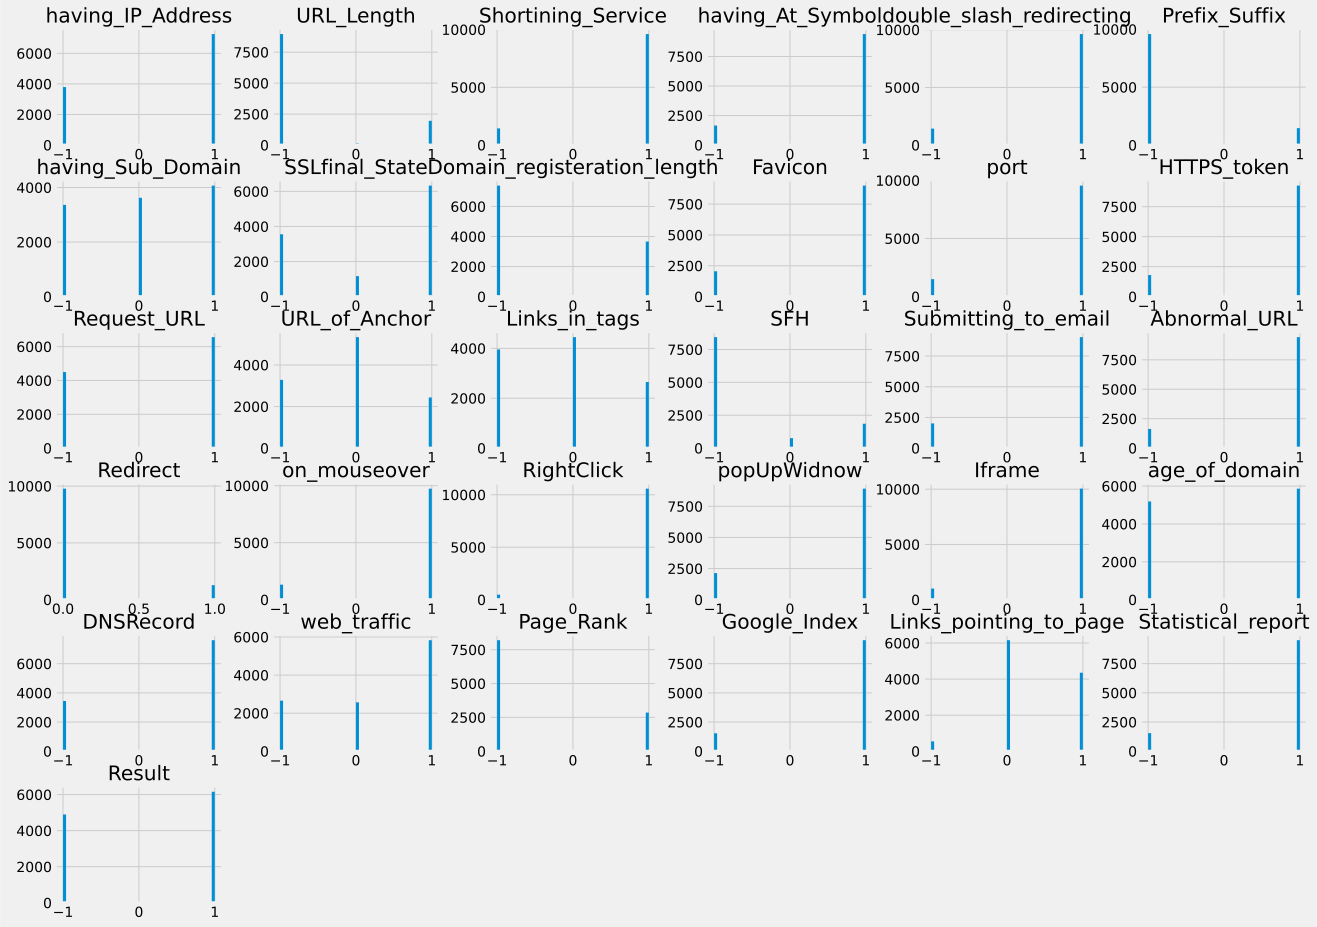
\includegraphics{project_files/figure-pdf/cell-5-output-1.svg}

}

\end{figure}

Creating correlation heatmap

\begin{Shaded}
\begin{Highlighting}[]
\NormalTok{plt.figure(figsize}\OperatorTok{=}\NormalTok{(}\DecValTok{15}\NormalTok{,}\DecValTok{13}\NormalTok{))}
\NormalTok{sns.heatmap(df.corr(), cmap}\OperatorTok{=}\StringTok{\textquotesingle{}coolwarm\textquotesingle{}}\NormalTok{)}
\NormalTok{plt.show()}
\end{Highlighting}
\end{Shaded}

\begin{figure}[H]

{\centering 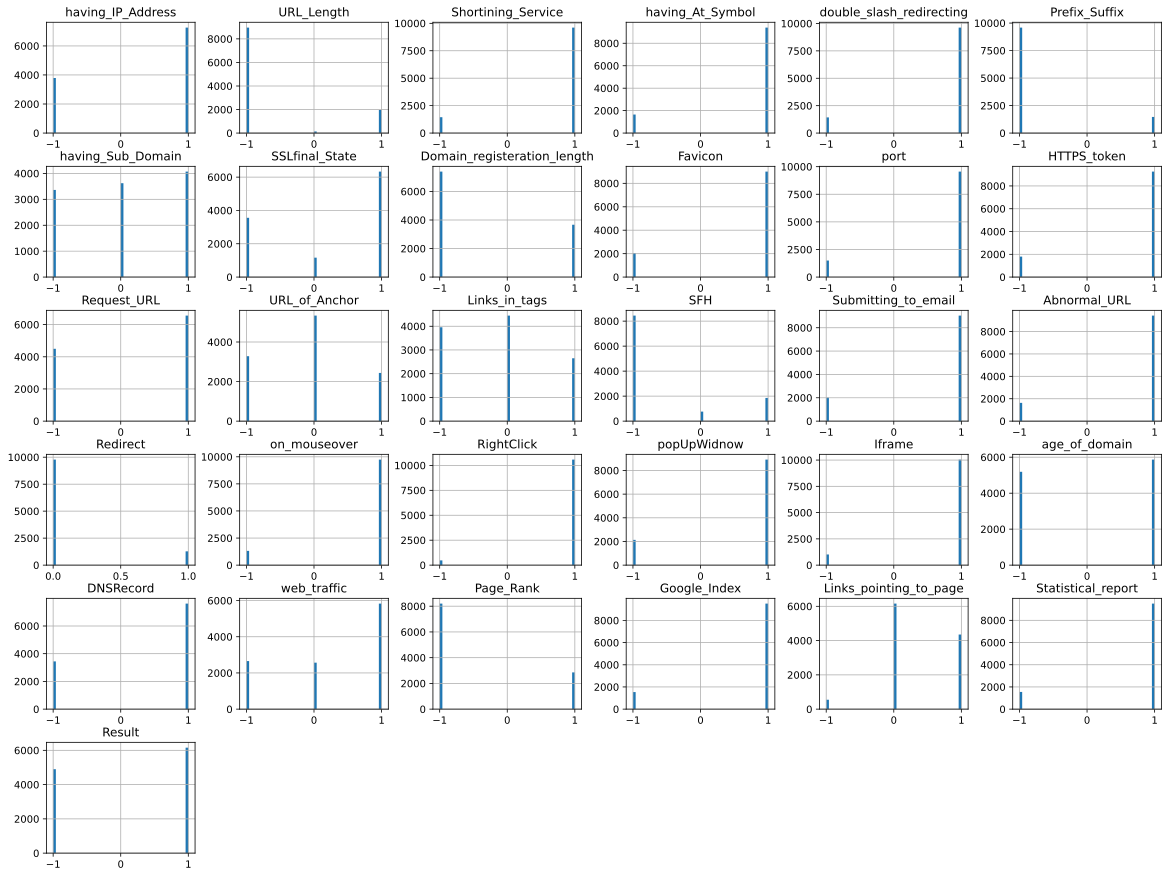
\includegraphics{project_files/figure-pdf/cell-6-output-1.svg}

}

\end{figure}

\hypertarget{prepping-the-data-to-be-used-in-ml-models}{%
\subsection{Prepping the data to be used in ML
models}\label{prepping-the-data-to-be-used-in-ml-models}}

Here we make sure that the data is clean and ready to use by the models

\begin{Shaded}
\begin{Highlighting}[]
\NormalTok{df.describe()}
\end{Highlighting}
\end{Shaded}

\begin{longtable}[]{@{}llllllllllllllllllllll@{}}
\toprule()
& having\_IP\_Address & URL\_Length & Shortining\_Service &
having\_At\_Symbol & double\_slash\_redirecting & Prefix\_Suffix &
having\_Sub\_Domain & SSLfinal\_State & Domain\_registeration\_length &
Favicon & ... & popUpWidnow & Iframe & age\_of\_domain & DNSRecord &
web\_traffic & Page\_Rank & Google\_Index & Links\_pointing\_to\_page &
Statistical\_report & Result \\
\midrule()
\endhead
count & 11055.000000 & 11055.000000 & 11055.000000 & 11055.000000 &
11055.000000 & 11055.000000 & 11055.000000 & 11055.000000 & 11055.000000
& 11055.000000 & ... & 11055.000000 & 11055.000000 & 11055.000000 &
11055.000000 & 11055.000000 & 11055.000000 & 11055.000000 & 11055.000000
& 11055.000000 & 11055.000000 \\
mean & 0.313795 & -0.633198 & 0.738761 & 0.700588 & 0.741474 & -0.734962
& 0.063953 & 0.250927 & -0.336771 & 0.628584 & ... & 0.613388 & 0.816915
& 0.061239 & 0.377114 & 0.287291 & -0.483673 & 0.721574 & 0.344007 &
0.719584 & 0.113885 \\
std & 0.949534 & 0.766095 & 0.673998 & 0.713598 & 0.671011 & 0.678139 &
0.817518 & 0.911892 & 0.941629 & 0.777777 & ... & 0.789818 & 0.576784 &
0.998168 & 0.926209 & 0.827733 & 0.875289 & 0.692369 & 0.569944 &
0.694437 & 0.993539 \\
min & -1.000000 & -1.000000 & -1.000000 & -1.000000 & -1.000000 &
-1.000000 & -1.000000 & -1.000000 & -1.000000 & -1.000000 & ... &
-1.000000 & -1.000000 & -1.000000 & -1.000000 & -1.000000 & -1.000000 &
-1.000000 & -1.000000 & -1.000000 & -1.000000 \\
25\% & -1.000000 & -1.000000 & 1.000000 & 1.000000 & 1.000000 &
-1.000000 & -1.000000 & -1.000000 & -1.000000 & 1.000000 & ... &
1.000000 & 1.000000 & -1.000000 & -1.000000 & 0.000000 & -1.000000 &
1.000000 & 0.000000 & 1.000000 & -1.000000 \\
50\% & 1.000000 & -1.000000 & 1.000000 & 1.000000 & 1.000000 & -1.000000
& 0.000000 & 1.000000 & -1.000000 & 1.000000 & ... & 1.000000 & 1.000000
& 1.000000 & 1.000000 & 1.000000 & -1.000000 & 1.000000 & 0.000000 &
1.000000 & 1.000000 \\
75\% & 1.000000 & -1.000000 & 1.000000 & 1.000000 & 1.000000 & -1.000000
& 1.000000 & 1.000000 & 1.000000 & 1.000000 & ... & 1.000000 & 1.000000
& 1.000000 & 1.000000 & 1.000000 & 1.000000 & 1.000000 & 1.000000 &
1.000000 & 1.000000 \\
max & 1.000000 & 1.000000 & 1.000000 & 1.000000 & 1.000000 & 1.000000 &
1.000000 & 1.000000 & 1.000000 & 1.000000 & ... & 1.000000 & 1.000000 &
1.000000 & 1.000000 & 1.000000 & 1.000000 & 1.000000 & 1.000000 &
1.000000 & 1.000000 \\
\bottomrule()
\end{longtable}

Because this dataset only contains boolean values \(\{-1, 0, 1\}\) we
don't have to do any further pre processing aside from omitting the
\texttt{index} column when training the models

\hypertarget{splitting-the-data-and-creating-trainingtesting-sets}{%
\subsection{Splitting the data and creating training/testing
sets}\label{splitting-the-data-and-creating-trainingtesting-sets}}

\begin{itemize}
\tightlist
\item
  X contains all of the criteria from index to statistical result
\item
  Y contains the actual result of whether a website is phishy or
  legitimate (-1 for phishy, 1 for legitimate)
\end{itemize}

\begin{Shaded}
\begin{Highlighting}[]
\CommentTok{\# importing packages for data preprocessing}
\ImportTok{from}\NormalTok{ sklearn.model\_selection }\ImportTok{import}\NormalTok{ train\_test\_split}

\NormalTok{X }\OperatorTok{=}\NormalTok{ df.iloc[:, :}\OperatorTok{{-}}\DecValTok{1}\NormalTok{]}
\NormalTok{y }\OperatorTok{=}\NormalTok{ df.iloc[:, }\OperatorTok{{-}}\DecValTok{1}\NormalTok{]}

\CommentTok{\# splitting the dataset into training and testing set with 80:20 ratio}
\NormalTok{X\_train, X\_test, y\_train, y\_test }\OperatorTok{=}\NormalTok{ train\_test\_split(X, y, test\_size}\OperatorTok{=}\FloatTok{0.2}\NormalTok{, random\_state}\OperatorTok{=}\DecValTok{42}\NormalTok{)}

\NormalTok{X.shape, y.shape}
\end{Highlighting}
\end{Shaded}

\begin{verbatim}
((11055, 30), (11055,))
\end{verbatim}

\hypertarget{training-the-models}{%
\section{Training the models}\label{training-the-models}}

Due to the nature of the dataset, it is clear that this is a supervised
machine learning task, which has two major types of problems,
classification, and regression. Because a website can be labeled either
phishy(-1) or legitimate(1) we are going to be using classifiers. The
supervised models I will be using are as follows:

\begin{itemize}
\tightlist
\item
  Decision Tree
\item
  Random Forest
\item
  Logistic Regression
\end{itemize}

\begin{Shaded}
\begin{Highlighting}[]
\CommentTok{\#importing packages for comparing accuracy}
\ImportTok{from}\NormalTok{ sklearn.metrics }\ImportTok{import}\NormalTok{ accuracy\_score}

\CommentTok{\# these lists will be used to store the accuracy of each model and will be converted into a single dataframe at the end}
\NormalTok{model }\OperatorTok{=}\NormalTok{ []}
\NormalTok{training\_accuracy }\OperatorTok{=}\NormalTok{ []}
\NormalTok{testing\_accuracy }\OperatorTok{=}\NormalTok{ []}

\KeywordTok{def}\NormalTok{ store\_accuracy(model\_name: }\BuiltInTok{str}\NormalTok{, train: }\BuiltInTok{float}\NormalTok{, test: }\BuiltInTok{float}\NormalTok{):}
    \CommentTok{"""}
\CommentTok{    This function stores the training and testing accuracy of each model in a list}
\CommentTok{    """}
\NormalTok{    model.append(model\_name)}
\NormalTok{    training\_accuracy.append(}\BuiltInTok{round}\NormalTok{(train, }\DecValTok{4}\NormalTok{))}
\NormalTok{    testing\_accuracy.append(}\BuiltInTok{round}\NormalTok{(test, }\DecValTok{4}\NormalTok{))}
\end{Highlighting}
\end{Shaded}

\hypertarget{decision-tree}{%
\subsection{Decision Tree}\label{decision-tree}}

Decision Trees are one of the most popular classification models when it
comes to boolean values like we're using here. A decision tree has a
flowchart-like structure, where each node is the question to an if-else
question, with each leaf node in the tree being the ending
classification.

In the case of this dataset, the leaf nodes of the decision tree would
be -1 for if the website is a phishing website and 1 if it's a
legitimate one

\begin{Shaded}
\begin{Highlighting}[]
\ImportTok{from}\NormalTok{ sklearn.tree }\ImportTok{import}\NormalTok{ DecisionTreeClassifier}

\CommentTok{\# creating a decision tree classifier}
\NormalTok{dt }\OperatorTok{=}\NormalTok{ DecisionTreeClassifier(random\_state}\OperatorTok{=}\DecValTok{42}\NormalTok{, max\_depth}\OperatorTok{=}\DecValTok{5}\NormalTok{)}

\CommentTok{\# training the model}
\NormalTok{dt.fit(X\_train, y\_train)}
\end{Highlighting}
\end{Shaded}

\begin{verbatim}
DecisionTreeClassifier(max_depth=5, random_state=42)
\end{verbatim}

\begin{Shaded}
\begin{Highlighting}[]
\CommentTok{\# predicting the values}
\NormalTok{y\_test\_tree }\OperatorTok{=}\NormalTok{ dt.predict(X\_test)}
\NormalTok{y\_train\_tree }\OperatorTok{=}\NormalTok{ dt.predict(X\_train)}
\end{Highlighting}
\end{Shaded}

\begin{Shaded}
\begin{Highlighting}[]
\CommentTok{\# calculating the accuracy}
\NormalTok{train\_accuracy }\OperatorTok{=}\NormalTok{ accuracy\_score(y\_train, y\_train\_tree)}
\NormalTok{test\_accuracy }\OperatorTok{=}\NormalTok{ accuracy\_score(y\_test, y\_test\_tree)}
\end{Highlighting}
\end{Shaded}

\hypertarget{evaluating-the-models}{%
\subsubsection{Evaluating the models}\label{evaluating-the-models}}

\begin{Shaded}
\begin{Highlighting}[]
\ImportTok{from}\NormalTok{ sklearn.metrics }\ImportTok{import}\NormalTok{ classification\_report}
\BuiltInTok{print}\NormalTok{(}\StringTok{"Decision Tree Accuracy on Training Set"}\NormalTok{)}
\BuiltInTok{print}\NormalTok{(classification\_report(y\_train, y\_train\_tree))}

\BuiltInTok{print}\NormalTok{(}\StringTok{"Accuracy on Training Set: "}\NormalTok{, }\BuiltInTok{round}\NormalTok{(train\_accuracy, }\DecValTok{4}\NormalTok{) }\OperatorTok{*} \DecValTok{100}\NormalTok{, }\StringTok{"\%"}\NormalTok{)}
\end{Highlighting}
\end{Shaded}

\begin{verbatim}
Decision Tree Accuracy on Training Set
              precision    recall  f1-score   support

          -1       0.96      0.86      0.91      3942
           1       0.90      0.97      0.93      4902

    accuracy                           0.92      8844
   macro avg       0.93      0.92      0.92      8844
weighted avg       0.92      0.92      0.92      8844

Accuracy on Training Set:  92.17999999999999 %
\end{verbatim}

\begin{Shaded}
\begin{Highlighting}[]
\BuiltInTok{print}\NormalTok{(}\StringTok{"Decision Tree Accuracy on Test Set"}\NormalTok{)}
\BuiltInTok{print}\NormalTok{(classification\_report(y\_test, y\_test\_tree))}

\BuiltInTok{print}\NormalTok{(}\StringTok{"Accuracy on Test Set: "}\NormalTok{, }\BuiltInTok{round}\NormalTok{(test\_accuracy, }\DecValTok{4}\NormalTok{) }\OperatorTok{*} \DecValTok{100}\NormalTok{, }\StringTok{"\%"}\NormalTok{)}
\end{Highlighting}
\end{Shaded}

\begin{verbatim}
Decision Tree Accuracy on Test Set
              precision    recall  f1-score   support

          -1       0.96      0.86      0.91       956
           1       0.90      0.98      0.94      1255

    accuracy                           0.92      2211
   macro avg       0.93      0.92      0.92      2211
weighted avg       0.93      0.92      0.92      2211

Accuracy on Test Set:  92.49000000000001 %
\end{verbatim}

\begin{Shaded}
\begin{Highlighting}[]
\CommentTok{\# storing results}
\NormalTok{store\_accuracy(}\StringTok{"Decision Tree"}\NormalTok{, }\BuiltInTok{round}\NormalTok{(train\_accuracy, }\DecValTok{4}\NormalTok{) }\OperatorTok{*} \DecValTok{100}\NormalTok{, }\BuiltInTok{round}\NormalTok{(test\_accuracy, }\DecValTok{4}\NormalTok{) }\OperatorTok{*} \DecValTok{100}\NormalTok{)}
\end{Highlighting}
\end{Shaded}

\hypertarget{visualizing-the-decision-tree}{%
\subsubsection{Visualizing the decision
tree}\label{visualizing-the-decision-tree}}

\begin{Shaded}
\begin{Highlighting}[]
\CommentTok{\# importing packages for visualizing the decision tree}
\ImportTok{from}\NormalTok{ sklearn.tree }\ImportTok{import}\NormalTok{ export\_graphviz}
\ImportTok{import}\NormalTok{ graphviz}

\CommentTok{\# visualizing the decision tree}
\NormalTok{dot }\OperatorTok{=}\NormalTok{ export\_graphviz(dt, out\_file}\OperatorTok{=}\StringTok{\textquotesingle{}figures/decision\_tree.gv\textquotesingle{}}\NormalTok{, feature\_names}\OperatorTok{=}\NormalTok{X.columns.values)}
\end{Highlighting}
\end{Shaded}

\begin{Shaded}
\begin{Highlighting}[]
\NormalTok{graphviz.Source.from\_file(}\StringTok{\textquotesingle{}figures/decision\_tree.gv\textquotesingle{}}\NormalTok{)}
\end{Highlighting}
\end{Shaded}

\begin{figure}[H]

{\centering 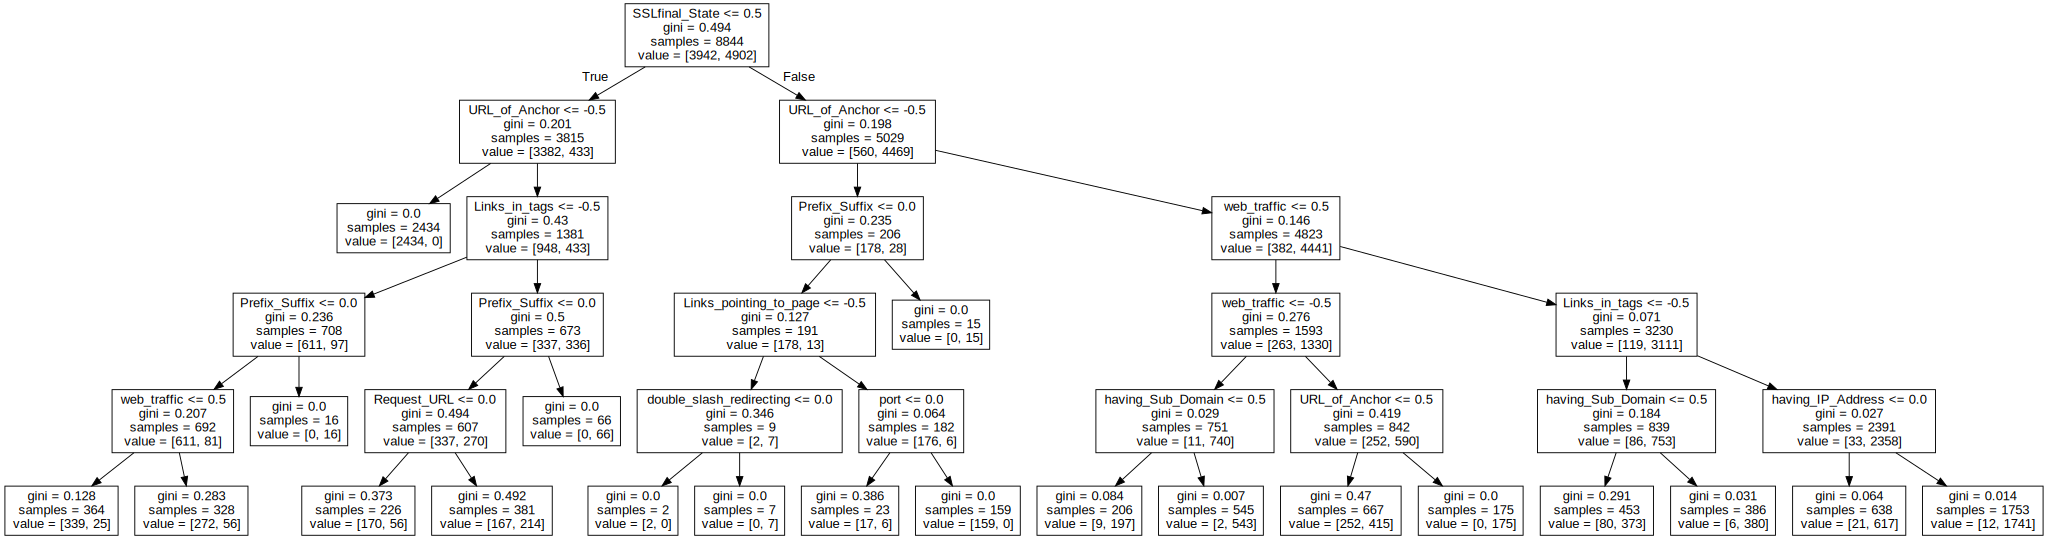
\includegraphics{project_files/figure-pdf/cell-17-output-1.svg}

}

\end{figure}

\begin{Shaded}
\begin{Highlighting}[]
\CommentTok{\#create feature importance plot}
\NormalTok{plt.figure(figsize}\OperatorTok{=}\NormalTok{(}\DecValTok{15}\NormalTok{, }\DecValTok{10}\NormalTok{))}
\NormalTok{features }\OperatorTok{=}\NormalTok{ X\_train.shape[}\DecValTok{1}\NormalTok{]}
\NormalTok{plt.barh(}\BuiltInTok{range}\NormalTok{(features), dt.feature\_importances\_, align}\OperatorTok{=}\StringTok{\textquotesingle{}center\textquotesingle{}}\NormalTok{)}
\NormalTok{plt.yticks(np.arange(features), X\_train.columns)}
\NormalTok{plt.xlabel(}\StringTok{"Feature Importance"}\NormalTok{)}
\NormalTok{plt.ylabel(}\StringTok{"Feature"}\NormalTok{)}
\NormalTok{plt.title(}\StringTok{"Decision Tree Feature Importance"}\NormalTok{)}
\NormalTok{plt.show()}
\end{Highlighting}
\end{Shaded}

\begin{figure}[H]

{\centering \includegraphics{project_files/figure-pdf/cell-18-output-1.svg}

}

\end{figure}

\hypertarget{identifying-false-positives-false-negatives-using-confusion-matrix}{%
\subsubsection{Identifying False Positives \& False Negatives Using
Confusion
Matrix}\label{identifying-false-positives-false-negatives-using-confusion-matrix}}

\begin{Shaded}
\begin{Highlighting}[]
\ImportTok{from}\NormalTok{ sklearn.metrics }\ImportTok{import}\NormalTok{ confusion\_matrix}

\CommentTok{\# creating a confusion matrix for the decision tree}
\NormalTok{cm }\OperatorTok{=}\NormalTok{ confusion\_matrix(y\_test, y\_test\_tree, labels}\OperatorTok{=}\NormalTok{[}\DecValTok{1}\NormalTok{, }\OperatorTok{{-}}\DecValTok{1}\NormalTok{])}
\NormalTok{sns.heatmap(cm, annot}\OperatorTok{=}\VariableTok{True}\NormalTok{, square}\OperatorTok{=}\VariableTok{True}\NormalTok{, fmt}\OperatorTok{=}\StringTok{\textquotesingle{}d\textquotesingle{}}\NormalTok{, cmap}\OperatorTok{=}\StringTok{\textquotesingle{}binary\textquotesingle{}}\NormalTok{)}
\NormalTok{plt.xlabel(}\StringTok{\textquotesingle{}true label\textquotesingle{}}\NormalTok{)}
\NormalTok{plt.ylabel(}\StringTok{\textquotesingle{}predicted label\textquotesingle{}}\NormalTok{)}
\NormalTok{plt.title(}\StringTok{\textquotesingle{}Decision Tree Confusion Matrix\textquotesingle{}}\NormalTok{)}
\NormalTok{plt.show()}
\NormalTok{plt.savefig(}\StringTok{\textquotesingle{}figures/decision\_tree\_confusion\_matrix.png\textquotesingle{}}\NormalTok{)}
\end{Highlighting}
\end{Shaded}

\begin{figure}[H]

{\centering \includegraphics{project_files/figure-pdf/cell-19-output-1.svg}

}

\end{figure}

\begin{verbatim}
<Figure size 640x480 with 0 Axes>
\end{verbatim}

\begin{itemize}
\tightlist
\item
  1225 websites were correctly labeled as legitimate\\
\item
  820 correctly labeled as phishing
\end{itemize}

\hypertarget{random-forest-classifier}{%
\subsection{Random Forest Classifier}\label{random-forest-classifier}}

A random forest is a classifer that is made up of an ensemble of
decision trees and each decision tree is slightly different than the
others. The main concept with decision trees is that while each tree
will do a pretty good job of predicting based on a training set, there
is a chance that it will overfit on some part of the data.

By building multiple decision trees and splitting up the data using
feature randomness, we create a ``forest'' of uncorrelated trees where
the prediction as a whole is more accurate than any individual tree

\begin{Shaded}
\begin{Highlighting}[]
\ImportTok{from}\NormalTok{ sklearn.ensemble }\ImportTok{import}\NormalTok{ RandomForestClassifier}

\CommentTok{\# creating a random forest classifier}
\NormalTok{rf }\OperatorTok{=}\NormalTok{ RandomForestClassifier(random\_state}\OperatorTok{=}\DecValTok{42}\NormalTok{, max\_depth}\OperatorTok{=}\DecValTok{5}\NormalTok{)}
\NormalTok{rf.fit(X\_train, y\_train)}
\end{Highlighting}
\end{Shaded}

\begin{verbatim}
RandomForestClassifier(max_depth=5, random_state=42)
\end{verbatim}

\begin{Shaded}
\begin{Highlighting}[]
\CommentTok{\# predicting the values}
\NormalTok{y\_test\_rf }\OperatorTok{=}\NormalTok{ rf.predict(X\_test)}
\NormalTok{y\_train\_rf }\OperatorTok{=}\NormalTok{ rf.predict(X\_train)}
\end{Highlighting}
\end{Shaded}

\begin{Shaded}
\begin{Highlighting}[]
\CommentTok{\# calculating the accuracy scores}
\NormalTok{rf\_train\_accuracy }\OperatorTok{=}\NormalTok{ accuracy\_score(y\_train, y\_train\_rf)}
\NormalTok{rf\_test\_accuracy }\OperatorTok{=}\NormalTok{ accuracy\_score(y\_test, y\_test\_rf)}
\end{Highlighting}
\end{Shaded}

\begin{Shaded}
\begin{Highlighting}[]
\CommentTok{\# displaying the classification report for the training set}
\BuiltInTok{print}\NormalTok{(}\StringTok{"Random Forest Accuracy on Training Set"}\NormalTok{)}
\BuiltInTok{print}\NormalTok{(classification\_report(y\_train, y\_train\_rf))}
\BuiltInTok{print}\NormalTok{(}\StringTok{"Accuracy on Training Set: "}\NormalTok{, }\BuiltInTok{round}\NormalTok{(rf\_train\_accuracy, }\DecValTok{4}\NormalTok{) }\OperatorTok{*} \DecValTok{100}\NormalTok{, }\StringTok{"\%"}\NormalTok{)}
\end{Highlighting}
\end{Shaded}

\begin{verbatim}
Random Forest Accuracy on Training Set
              precision    recall  f1-score   support

          -1       0.95      0.90      0.92      3942
           1       0.92      0.96      0.94      4902

    accuracy                           0.93      8844
   macro avg       0.93      0.93      0.93      8844
weighted avg       0.93      0.93      0.93      8844

Accuracy on Training Set:  93.08999999999999 %
\end{verbatim}

\begin{Shaded}
\begin{Highlighting}[]
\BuiltInTok{print}\NormalTok{(}\StringTok{"Random Forest Accuracy on Test Set"}\NormalTok{)}
\BuiltInTok{print}\NormalTok{(classification\_report(y\_test, y\_test\_rf))}
\BuiltInTok{print}\NormalTok{(}\StringTok{"Accuracy on Test Set: "}\NormalTok{, }\BuiltInTok{round}\NormalTok{(rf\_test\_accuracy, }\DecValTok{4}\NormalTok{) }\OperatorTok{*} \DecValTok{100}\NormalTok{, }\StringTok{"\%"}\NormalTok{)}
\end{Highlighting}
\end{Shaded}

\begin{verbatim}
Random Forest Accuracy on Test Set
              precision    recall  f1-score   support

          -1       0.95      0.90      0.92       956
           1       0.93      0.96      0.94      1255

    accuracy                           0.93      2211
   macro avg       0.94      0.93      0.93      2211
weighted avg       0.93      0.93      0.93      2211

Accuracy on Test Set:  93.44 %
\end{verbatim}

\begin{Shaded}
\begin{Highlighting}[]
\CommentTok{\# storing results}
\NormalTok{store\_accuracy(}\StringTok{"Random Forest"}\NormalTok{, }\BuiltInTok{round}\NormalTok{(rf\_train\_accuracy, }\DecValTok{4}\NormalTok{) }\OperatorTok{*} \DecValTok{100}\NormalTok{, }\BuiltInTok{round}\NormalTok{(rf\_test\_accuracy, }\DecValTok{4}\NormalTok{) }\OperatorTok{*} \DecValTok{100}\NormalTok{)}
\end{Highlighting}
\end{Shaded}

\begin{Shaded}
\begin{Highlighting}[]
\CommentTok{\# checking the feature importance}
\NormalTok{plt.figure(figsize}\OperatorTok{=}\NormalTok{(}\DecValTok{15}\NormalTok{, }\DecValTok{10}\NormalTok{))}
\NormalTok{features }\OperatorTok{=}\NormalTok{ X\_train.shape[}\DecValTok{1}\NormalTok{]}
\NormalTok{plt.barh(}\BuiltInTok{range}\NormalTok{(features), rf.feature\_importances\_, align}\OperatorTok{=}\StringTok{\textquotesingle{}center\textquotesingle{}}\NormalTok{)}
\NormalTok{plt.yticks(np.arange(features), X\_train.columns)}
\NormalTok{plt.xlabel(}\StringTok{"Feature Importance"}\NormalTok{)}
\NormalTok{plt.ylabel(}\StringTok{"Feature"}\NormalTok{)}
\NormalTok{plt.title(}\StringTok{"Random Forest Feature Importance"}\NormalTok{)}
\NormalTok{plt.show()}
\end{Highlighting}
\end{Shaded}

\begin{figure}[H]

{\centering \includegraphics{project_files/figure-pdf/cell-26-output-1.svg}

}

\end{figure}

\hypertarget{identifying-false-positves-and-false-negatives}{%
\subsubsection{Identifying False Positves and False
negatives}\label{identifying-false-positves-and-false-negatives}}

\begin{Shaded}
\begin{Highlighting}[]
\CommentTok{\# creating a confusion matrix for the random forest}
\NormalTok{cm }\OperatorTok{=}\NormalTok{ confusion\_matrix(y\_test, y\_test\_rf, labels}\OperatorTok{=}\NormalTok{[}\DecValTok{1}\NormalTok{, }\OperatorTok{{-}}\DecValTok{1}\NormalTok{])}
\NormalTok{sns.heatmap(cm, annot}\OperatorTok{=}\VariableTok{True}\NormalTok{, square}\OperatorTok{=}\VariableTok{True}\NormalTok{, fmt}\OperatorTok{=}\StringTok{\textquotesingle{}d\textquotesingle{}}\NormalTok{, cmap}\OperatorTok{=}\StringTok{\textquotesingle{}binary\textquotesingle{}}\NormalTok{)}
\NormalTok{plt.xlabel(}\StringTok{\textquotesingle{}true label\textquotesingle{}}\NormalTok{)}
\NormalTok{plt.ylabel(}\StringTok{\textquotesingle{}predicted label\textquotesingle{}}\NormalTok{)}
\NormalTok{plt.title(}\StringTok{\textquotesingle{}Random Forest Confusion Matrix\textquotesingle{}}\NormalTok{)}
\NormalTok{plt.show()}
\NormalTok{plt.savefig(}\StringTok{\textquotesingle{}figures/random\_forest\_confusion\_matrix.png\textquotesingle{}}\NormalTok{)}
\end{Highlighting}
\end{Shaded}

\begin{figure}[H]

{\centering \includegraphics{project_files/figure-pdf/cell-27-output-1.svg}

}

\end{figure}

\begin{verbatim}
<Figure size 640x480 with 0 Axes>
\end{verbatim}

\begin{itemize}
\tightlist
\item
  1207 websites were correctly labeled as legitimate
\item
  859 websites were correctly labeled as phishing
\end{itemize}

\hypertarget{logistic-regression}{%
\subsection{Logistic Regression}\label{logistic-regression}}

\begin{Shaded}
\begin{Highlighting}[]
\CommentTok{\# importing packages for logistic regression}
\ImportTok{from}\NormalTok{ sklearn.linear\_model }\ImportTok{import}\NormalTok{ LogisticRegression}

\CommentTok{\# creating a logistic regression model for binary classification}
\NormalTok{lr }\OperatorTok{=}\NormalTok{ LogisticRegression(random\_state}\OperatorTok{=}\DecValTok{42}\NormalTok{, max\_iter}\OperatorTok{=}\DecValTok{1000}\NormalTok{)}
\NormalTok{lr.fit(X\_train, y\_train)}
\end{Highlighting}
\end{Shaded}

\begin{verbatim}
LogisticRegression(max_iter=1000, random_state=42)
\end{verbatim}

\begin{Shaded}
\begin{Highlighting}[]
\CommentTok{\# predicting the values}
\NormalTok{y\_test\_lr }\OperatorTok{=}\NormalTok{ lr.predict(X\_test)}
\NormalTok{y\_train\_lr }\OperatorTok{=}\NormalTok{ lr.predict(X\_train)}
\end{Highlighting}
\end{Shaded}

\begin{Shaded}
\begin{Highlighting}[]
\CommentTok{\# calculating the accuracy scores}
\NormalTok{lr\_train\_accuracy }\OperatorTok{=}\NormalTok{ accuracy\_score(y\_train, y\_train\_lr)}
\NormalTok{lr\_test\_accuracy }\OperatorTok{=}\NormalTok{ accuracy\_score(y\_test, y\_test\_lr)}
\end{Highlighting}
\end{Shaded}

\begin{Shaded}
\begin{Highlighting}[]
\CommentTok{\# displaying the classification report for the training set}
\BuiltInTok{print}\NormalTok{(}\StringTok{"Logistic Regression Accuracy on Training Set"}\NormalTok{)}
\BuiltInTok{print}\NormalTok{(classification\_report(y\_train, y\_train\_lr))}
\BuiltInTok{print}\NormalTok{(}\StringTok{"Accuracy on Training Set: "}\NormalTok{, }\BuiltInTok{round}\NormalTok{(lr\_train\_accuracy, }\DecValTok{4}\NormalTok{) }\OperatorTok{*} \DecValTok{100}\NormalTok{, }\StringTok{"\%"}\NormalTok{)}
\end{Highlighting}
\end{Shaded}

\begin{verbatim}
Logistic Regression Accuracy on Training Set
              precision    recall  f1-score   support

          -1       0.93      0.91      0.92      3942
           1       0.93      0.95      0.94      4902

    accuracy                           0.93      8844
   macro avg       0.93      0.93      0.93      8844
weighted avg       0.93      0.93      0.93      8844

Accuracy on Training Set:  92.94 %
\end{verbatim}

\begin{Shaded}
\begin{Highlighting}[]
\CommentTok{\# displaying the classification report for the test set}
\BuiltInTok{print}\NormalTok{(}\StringTok{"Logistic Regression Accuracy on Test Set"}\NormalTok{)}
\BuiltInTok{print}\NormalTok{(classification\_report(y\_test, y\_test\_lr))}
\BuiltInTok{print}\NormalTok{(}\StringTok{"Accuracy on Test Set: "}\NormalTok{, }\BuiltInTok{round}\NormalTok{(lr\_test\_accuracy, }\DecValTok{4}\NormalTok{) }\OperatorTok{*} \DecValTok{100}\NormalTok{, }\StringTok{"\%"}\NormalTok{)}
\end{Highlighting}
\end{Shaded}

\begin{verbatim}
Logistic Regression Accuracy on Test Set
              precision    recall  f1-score   support

          -1       0.92      0.90      0.91       956
           1       0.93      0.94      0.93      1255

    accuracy                           0.92      2211
   macro avg       0.92      0.92      0.92      2211
weighted avg       0.92      0.92      0.92      2211

Accuracy on Test Set:  92.4 %
\end{verbatim}

\begin{Shaded}
\begin{Highlighting}[]
\CommentTok{\# storing results}
\NormalTok{store\_accuracy(}\StringTok{"Logistic Regression"}\NormalTok{, }\BuiltInTok{round}\NormalTok{(lr\_train\_accuracy, }\DecValTok{4}\NormalTok{) }\OperatorTok{*} \DecValTok{100}\NormalTok{, }\BuiltInTok{round}\NormalTok{(lr\_test\_accuracy, }\DecValTok{4}\NormalTok{) }\OperatorTok{*} \DecValTok{100}\NormalTok{)}
\end{Highlighting}
\end{Shaded}

\begin{Shaded}
\begin{Highlighting}[]
\CommentTok{\# creating a confusion matrix for the logistic regression}
\NormalTok{cm }\OperatorTok{=}\NormalTok{ confusion\_matrix(y\_test, y\_test\_lr, labels}\OperatorTok{=}\NormalTok{[}\DecValTok{1}\NormalTok{, }\OperatorTok{{-}}\DecValTok{1}\NormalTok{])}
\NormalTok{sns.heatmap(cm, annot}\OperatorTok{=}\VariableTok{True}\NormalTok{, square}\OperatorTok{=}\VariableTok{True}\NormalTok{, fmt}\OperatorTok{=}\StringTok{\textquotesingle{}d\textquotesingle{}}\NormalTok{, cmap}\OperatorTok{=}\StringTok{\textquotesingle{}binary\textquotesingle{}}\NormalTok{)}
\NormalTok{plt.xlabel(}\StringTok{\textquotesingle{}true label\textquotesingle{}}\NormalTok{)}
\NormalTok{plt.ylabel(}\StringTok{\textquotesingle{}predicted label\textquotesingle{}}\NormalTok{)}
\NormalTok{plt.title(}\StringTok{\textquotesingle{}Logistic Regression Confusion Matrix\textquotesingle{}}\NormalTok{)}
\NormalTok{plt.show()}
\NormalTok{plt.savefig(}\StringTok{\textquotesingle{}figures/logistic\_regression\_confusion\_matrix.png\textquotesingle{}}\NormalTok{)}
\end{Highlighting}
\end{Shaded}

\begin{figure}[H]

{\centering \includegraphics{project_files/figure-pdf/cell-34-output-1.svg}

}

\end{figure}

\begin{verbatim}
<Figure size 640x480 with 0 Axes>
\end{verbatim}

\begin{itemize}
\tightlist
\item
  1179 websites were correctly labeled as legitimate
\item
  864 websites were correctly labeled as phishing
\end{itemize}

\hypertarget{supervised-vector-machine-svm-classification}{%
\subsection{Supervised Vector Machine (SVM
Classification)}\label{supervised-vector-machine-svm-classification}}

\hypertarget{creating-and-fitting-the-model}{%
\subsubsection{Creating and fitting the
model}\label{creating-and-fitting-the-model}}

\begin{Shaded}
\begin{Highlighting}[]
\CommentTok{\# importing packages for SVM classifer}
\ImportTok{from}\NormalTok{ sklearn.svm }\ImportTok{import}\NormalTok{ SVC}

\CommentTok{\# creating a SVM classifier}
\NormalTok{svm }\OperatorTok{=}\NormalTok{ SVC(kernel}\OperatorTok{=}\StringTok{\textquotesingle{}linear\textquotesingle{}}\NormalTok{, C}\OperatorTok{=}\FloatTok{1.0}\NormalTok{,random\_state}\OperatorTok{=}\DecValTok{42}\NormalTok{) }\CommentTok{\# using linear kernel with C=1.0}

\CommentTok{\# training the model}
\NormalTok{svm.fit(X\_train, y\_train)}
\end{Highlighting}
\end{Shaded}

\begin{verbatim}
SVC(kernel='linear', random_state=42)
\end{verbatim}

\begin{Shaded}
\begin{Highlighting}[]
\CommentTok{\# predicting the values}
\NormalTok{y\_test\_svm }\OperatorTok{=}\NormalTok{ svm.predict(X\_test)}
\NormalTok{y\_train\_svm }\OperatorTok{=}\NormalTok{ svm.predict(X\_train)}
\end{Highlighting}
\end{Shaded}

\begin{Shaded}
\begin{Highlighting}[]
\CommentTok{\# calculating the accuracy scores}
\NormalTok{svm\_train\_accuracy }\OperatorTok{=}\NormalTok{ accuracy\_score(y\_train, y\_train\_svm)}
\NormalTok{svm\_test\_accuracy }\OperatorTok{=}\NormalTok{ accuracy\_score(y\_test, y\_test\_svm)}
\end{Highlighting}
\end{Shaded}

\begin{Shaded}
\begin{Highlighting}[]
\CommentTok{\# displaying the classification report for the training set}
\BuiltInTok{print}\NormalTok{(}\StringTok{"SVM Accuracy on Training Set"}\NormalTok{)}
\BuiltInTok{print}\NormalTok{(classification\_report(y\_train, y\_train\_svm))}
\BuiltInTok{print}\NormalTok{(}\StringTok{"Accuracy on Training Set: "}\NormalTok{, }\BuiltInTok{round}\NormalTok{(svm\_train\_accuracy, }\DecValTok{4}\NormalTok{) }\OperatorTok{*} \DecValTok{100}\NormalTok{, }\StringTok{"\%"}\NormalTok{)}
\end{Highlighting}
\end{Shaded}

\begin{verbatim}
SVM Accuracy on Training Set
              precision    recall  f1-score   support

          -1       0.93      0.91      0.92      3942
           1       0.93      0.95      0.94      4902

    accuracy                           0.93      8844
   macro avg       0.93      0.93      0.93      8844
weighted avg       0.93      0.93      0.93      8844

Accuracy on Training Set:  92.84 %
\end{verbatim}

\begin{Shaded}
\begin{Highlighting}[]
\CommentTok{\# displaying the classification report for the test set}
\BuiltInTok{print}\NormalTok{(}\StringTok{"SVM Accuracy on Test Set"}\NormalTok{)}
\BuiltInTok{print}\NormalTok{(classification\_report(y\_test, y\_test\_svm))}
\BuiltInTok{print}\NormalTok{(}\StringTok{"Accuracy on Test Set: "}\NormalTok{, }\BuiltInTok{round}\NormalTok{(svm\_test\_accuracy, }\DecValTok{4}\NormalTok{) }\OperatorTok{*} \DecValTok{100}\NormalTok{, }\StringTok{"\%"}\NormalTok{)}
\end{Highlighting}
\end{Shaded}

\begin{verbatim}
SVM Accuracy on Test Set
              precision    recall  f1-score   support

          -1       0.93      0.90      0.92       956
           1       0.93      0.95      0.94      1255

    accuracy                           0.93      2211
   macro avg       0.93      0.93      0.93      2211
weighted avg       0.93      0.93      0.93      2211

Accuracy on Test Set:  92.85 %
\end{verbatim}

\begin{Shaded}
\begin{Highlighting}[]
\CommentTok{\# storing results}
\NormalTok{store\_accuracy(}\StringTok{"SVM"}\NormalTok{, }\BuiltInTok{round}\NormalTok{(svm\_train\_accuracy, }\DecValTok{4}\NormalTok{) }\OperatorTok{*} \DecValTok{100}\NormalTok{, }\BuiltInTok{round}\NormalTok{(svm\_test\_accuracy, }\DecValTok{4}\NormalTok{) }\OperatorTok{*} \DecValTok{100}\NormalTok{)}
\end{Highlighting}
\end{Shaded}

\hypertarget{identifying-false-positives-and-negatives}{%
\subsubsection{Identifying False Positives and
Negatives}\label{identifying-false-positives-and-negatives}}

\begin{Shaded}
\begin{Highlighting}[]
\CommentTok{\# creating a confusion matrix for the SVM}
\NormalTok{cm }\OperatorTok{=}\NormalTok{ confusion\_matrix(y\_test, y\_test\_svm, labels}\OperatorTok{=}\NormalTok{[}\DecValTok{1}\NormalTok{, }\OperatorTok{{-}}\DecValTok{1}\NormalTok{])}
\NormalTok{sns.heatmap(cm, annot}\OperatorTok{=}\VariableTok{True}\NormalTok{, square}\OperatorTok{=}\VariableTok{True}\NormalTok{, fmt}\OperatorTok{=}\StringTok{\textquotesingle{}d\textquotesingle{}}\NormalTok{, cmap}\OperatorTok{=}\StringTok{\textquotesingle{}binary\textquotesingle{}}\NormalTok{)}
\NormalTok{plt.xlabel(}\StringTok{\textquotesingle{}true label\textquotesingle{}}\NormalTok{)}
\NormalTok{plt.ylabel(}\StringTok{\textquotesingle{}predicted label\textquotesingle{}}\NormalTok{)}
\NormalTok{plt.title(}\StringTok{\textquotesingle{}SVM Confusion Matrix\textquotesingle{}}\NormalTok{)}
\NormalTok{plt.show()}
\NormalTok{plt.savefig(}\StringTok{\textquotesingle{}figures/svm\_confusion\_matrix.png\textquotesingle{}}\NormalTok{)}
\end{Highlighting}
\end{Shaded}

\begin{figure}[H]

{\centering \includegraphics{project_files/figure-pdf/cell-41-output-1.svg}

}

\end{figure}

\begin{verbatim}
<Figure size 640x480 with 0 Axes>
\end{verbatim}

\begin{itemize}
\tightlist
\item
  1192 websites were correctly identified as legitimate
\item
  861 websites were correctly identified as phishing
\end{itemize}

\hypertarget{comparing-all-the-models}{%
\section{Comparing all the Models}\label{comparing-all-the-models}}

\begin{Shaded}
\begin{Highlighting}[]
\CommentTok{\# creating dataframe with all the results}
\NormalTok{results }\OperatorTok{=}\NormalTok{ pd.DataFrame(\{}\StringTok{"ML Model"}\NormalTok{: model, }\StringTok{"Training Accuracy"}\NormalTok{: training\_accuracy, }\StringTok{"Test Accuracy"}\NormalTok{: testing\_accuracy\})}
\NormalTok{results}
\end{Highlighting}
\end{Shaded}

\begin{longtable}[]{@{}llll@{}}
\toprule()
& ML Model & Training Accuracy & Test Accuracy \\
\midrule()
\endhead
0 & Decision Tree & 92.18 & 92.49 \\
1 & Random Forest & 93.09 & 93.44 \\
2 & Logistic Regression & 92.94 & 92.40 \\
3 & SVM & 92.84 & 92.85 \\
\bottomrule()
\end{longtable}

\begin{Shaded}
\begin{Highlighting}[]
\CommentTok{\# sorting the results by accuracy}
\NormalTok{results.sort\_values(by}\OperatorTok{=}\NormalTok{[}\StringTok{\textquotesingle{}Training Accuracy\textquotesingle{}}\NormalTok{, }\StringTok{\textquotesingle{}Test Accuracy\textquotesingle{}}\NormalTok{], ascending}\OperatorTok{=}\VariableTok{False}\NormalTok{)}
\end{Highlighting}
\end{Shaded}

\begin{longtable}[]{@{}llll@{}}
\toprule()
& ML Model & Training Accuracy & Test Accuracy \\
\midrule()
\endhead
1 & Random Forest & 93.09 & 93.44 \\
2 & Logistic Regression & 92.94 & 92.40 \\
3 & SVM & 92.84 & 92.85 \\
0 & Decision Tree & 92.18 & 92.49 \\
\bottomrule()
\end{longtable}

Out of these 4 models we can see that random forest is the model that
will best fit the given dataset

\begin{Shaded}
\begin{Highlighting}[]
\CommentTok{\# plotting the results in a bar chart, one bar for training accuracy and one for test accuracy}
\NormalTok{plt.figure(figsize}\OperatorTok{=}\NormalTok{(}\DecValTok{40}\NormalTok{, }\DecValTok{80}\NormalTok{))}
\NormalTok{plt.style.use(}\StringTok{\textquotesingle{}fivethirtyeight\textquotesingle{}}\NormalTok{)}
\NormalTok{labels }\OperatorTok{=}\NormalTok{ results[}\StringTok{\textquotesingle{}ML Model\textquotesingle{}}\NormalTok{]}
\NormalTok{x }\OperatorTok{=}\NormalTok{ np.arange(}\BuiltInTok{len}\NormalTok{(labels))}
\NormalTok{width }\OperatorTok{=} \FloatTok{0.25}
\NormalTok{fig, ax }\OperatorTok{=}\NormalTok{ plt.subplots()}
\NormalTok{rects1 }\OperatorTok{=}\NormalTok{ ax.bar(x }\OperatorTok{{-}}\NormalTok{ width}\OperatorTok{/}\DecValTok{2}\NormalTok{, training\_accuracy, width, label}\OperatorTok{=}\StringTok{\textquotesingle{}Training\textquotesingle{}}\NormalTok{)}
\NormalTok{rects2 }\OperatorTok{=}\NormalTok{ ax.bar(x }\OperatorTok{+}\NormalTok{ width}\OperatorTok{/}\DecValTok{2}\NormalTok{, testing\_accuracy, width, label}\OperatorTok{=}\StringTok{\textquotesingle{}Testing\textquotesingle{}}\NormalTok{)}



\NormalTok{ax.set\_ylabel(}\StringTok{\textquotesingle{}Accuracy (\%)\textquotesingle{}}\NormalTok{)}
\NormalTok{ax.set\_xlabel(}\StringTok{\textquotesingle{}ML Model\textquotesingle{}}\NormalTok{)}
\NormalTok{ax.set\_title(}\StringTok{\textquotesingle{}Accuracy of Different Models\textquotesingle{}}\NormalTok{)}
\NormalTok{ax.set\_xticks(x, labels)}
\NormalTok{ax.set\_xticklabels(labels)}
\NormalTok{ax.set\_ylim(}\DecValTok{75}\NormalTok{, }\DecValTok{100}\NormalTok{)}
\NormalTok{ax.legend()}

\NormalTok{fig.tight\_layout()}

\NormalTok{plt.show()}
\end{Highlighting}
\end{Shaded}

\begin{verbatim}
<Figure size 4000x8000 with 0 Axes>
\end{verbatim}

\begin{figure}[H]

{\centering \includegraphics{project_files/figure-pdf/cell-44-output-2.svg}

}

\end{figure}

Looking at the graph and seeing that the bars are mostly even we can
come to the conclusion that the models were properly fit from the data



\end{document}
